\normaltrue
\correctiontrue

%\UPSTIidClasse{11} % 11 sup, 12 spé
%\newcommand{\UPSTIidClasse}{12}


\exer{Mouvement TT -- $\star$ \label{B2:13:03}}
\setcounter{numques}{0}
\UPSTIcompetence[2]{C2-05}
\UPSTIcompetence[2]{B2-13}
\index{Compétence C2-05}
\index{Compétence B2-13}
\index{Mécanisme à 2 translations}
\ifcorrection
\else
\textbf{Pas de corrigé pour cet exercice.}
\fi

\ifprof
\else
Soit le mécanisme suivant. On note $\vect{AB}=\lambda(t)\vect{i_0}$ et $\vect{BC}=\mu(t)\vect{j_0}$.
\begin{center}
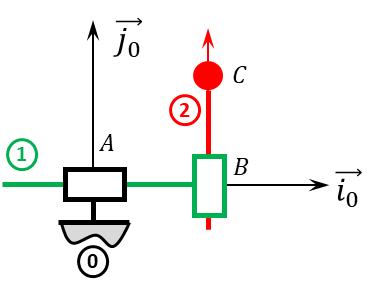
\includegraphics[width=.6\linewidth]{03_TT_01}
\end{center}
\fi

\question{Quel est le mouvement de \textbf{2} par rapport à~\textbf{0}.}
\ifprof ~\\
Le point $C$ a un mouvement quelconque dans le plan $\left(A,\vi{0},\vj{0}\right)$.
\else
\fi

\question{Donner l'équation du mouvement du point $C$ dans le mouvement de \textbf{2} par rapport à~\textbf{0}.}
\ifprof ~\\
On  a $\vect{AC}=\lambda(t)\vect{i_0}+\mu(t)\vect{j_0}$ et donc, on a directement 
$\left\{
\begin{array}{l}
x_C(t)= \lambda(t) \\
y_C(t)= \mu(t)\\
z_C(t)= 0\\
\end{array}
\right.
$ dans le repère $\repere{A}{i_0}{j_0}{k_0}$.

\else
\fi

On souhaite que le point $C$ réalise un cercle de centre $A$ et de rayon $R=\SI{10}{cm}$. 

\question{Donner les expressions de $\lambda(t)$ et $\mu(t)$ permettant la réalisation de cette trajectoire à la vitesse $v=\SI{0,01}{m.s^{-1}}$ en fonction de $v$, $R$ et du temps}
\ifprof  ~\\
Exprimons la trajectoire du point $C$ : $\vect{AC}=R\vect{e_r} = R\cos\theta(t) \vi{0}+ R\sin\theta(t)  \vj{0}$. Par identification 
$ \lambda(t) = R\cos\theta(t)$ et $\mu(t) = R\sin\theta(t)$.

Par ailleurs la vitesse du point $C$ est donnée par $\vectv{C}{2}{0}=\deriv{\vect{AC}}{\rep{0}} = R\dot{\theta}\vect{e_\theta}$. 
On a donc $v=R\dot{\theta}(t)$. Par intégration, $ \theta(t)=\dfrac{v}{R}t$ (avec $\theta(t)=\SI{0}{rad}$ pour $t=\SI{0}{s}$). Au final, 
$\left\{
\begin{array}{l}
\lambda(t) = R\cos\left( \dfrac{v}{R}t\right)\\
\mu(t) = R\sin\left( \dfrac{v}{R}t\right)\\
\end{array}
\right.
$.

\else
\fi


\question{En utilisant Python, tracer $\lambda(t)$, $\mu(t)$ et la trajectoire générée.}
\ifprof
~\\
\noindent\rule{\linewidth}{.1mm}
\begin{lstlisting}
import numpy as np
import matplotlib.pyplot as plt
import math as m
R = 0.1 # m
v = 0.01 # m.s-1 

# Temps pour faire un tour 
T = 2*m.pi*R/v

les_t = np.linspace(0,T,200)
les_lambda = R*np.cos(v/R*les_t)
les_mu = R*np.sin(v/R*les_t)
plt.grid()
plt.plot(les_t,les_lambda,label="$\\lambda(t)$")
plt.plot(les_t,les_mu,label="$\\mu(t)$")
plt.xlabel("Temps ($s$)")
plt.ylabel("Position ($m$)")
plt.legend()
#plt.show()
plt.savefig("03_TT_01_c.pdf")
plt.cla()

plt.grid()
plt.axis("equal")
plt.plot(les_lambda,les_mu,label="Trajectoire de $C$")
plt.legend()
#plt.show()
plt.savefig("03_TT_02_c.pdf")
\end{lstlisting}
\noindent\rule{\linewidth}{.1mm}

\begin{minipage}[c]{.45\linewidth}
\begin{center}
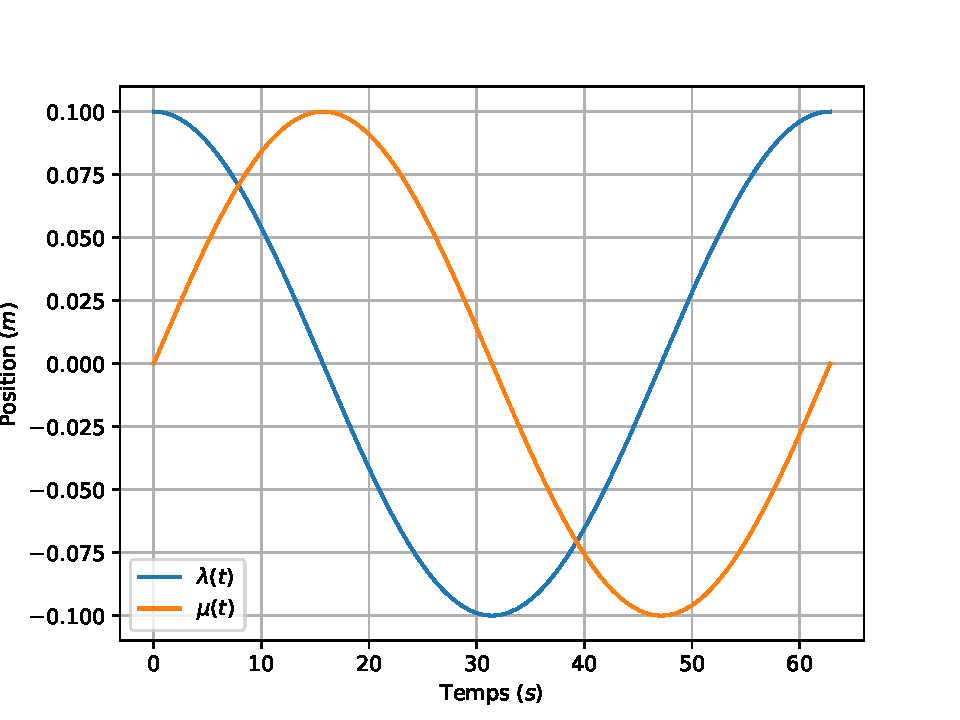
\includegraphics[width=.8\linewidth]{03_TT_01_c}
\end{center}
\end{minipage} \hfill
\begin{minipage}[c]{.45\linewidth}
\begin{center}
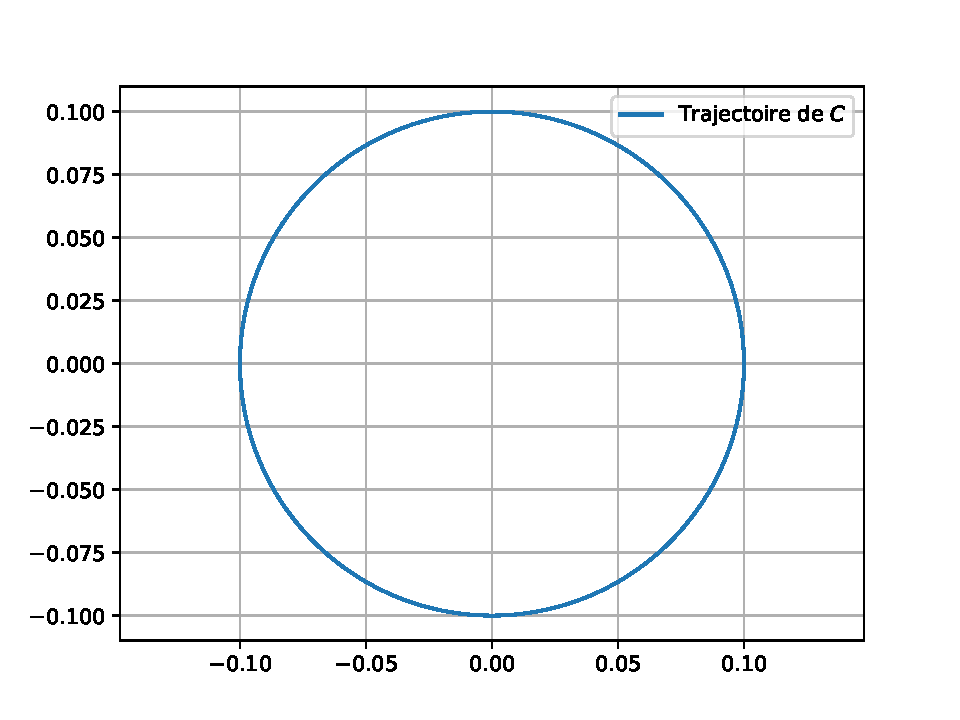
\includegraphics[width=.8\linewidth]{03_TT_02_c}
\end{center}
\end{minipage} 
\else
\fi


\ifprof
\else
\begin{flushright}
\footnotesize{Corrigé  voir \ref{B2:13:03}.}
\end{flushright}%
\fi


